\documentclass[10pt,a4paper]{article}

\usepackage[margin=1.55cm,footskip=1.05cm]{geometry}
\usepackage[T1]{fontenc}
\usepackage{lmodern}
\usepackage{microtype}
\usepackage{booktabs}
\usepackage{tabularx}
\usepackage{array}
\usepackage{enumitem}
\usepackage{xcolor}
\usepackage{tikz}
\usetikzlibrary{arrows.meta,positioning,calc}
\usepackage{float}
\usepackage{caption}
\usepackage{titlesec}
\usepackage{fancyhdr}
\usepackage{lastpage}
\usepackage[hidelinks]{hyperref}

\newcolumntype{Y}{>{\raggedright\arraybackslash}X}
\captionsetup{font=footnotesize,labelfont={bf,sf},skip=4pt}
\setlength{\intextsep}{4pt plus 1pt minus 1pt}
\setlength{\textfloatsep}{4pt plus 1pt minus 1pt}
\setlist[enumerate]{leftmargin=1.3em,itemsep=0.15em,topsep=0.25em,parsep=0pt}
\pagestyle{fancy}
\fancyhf{}
\fancyfoot[L]{\footnotesize CS6.403 AutoSE \textperiodcentered\ HarnessSpec mid-submission}
\fancyfoot[R]{\footnotesize \thepage\ / \pageref{LastPage}}
\renewcommand{\headrulewidth}{0pt}
\renewcommand{\footrulewidth}{0.3pt}
\linespread{0.96}
\titlespacing*{\section}{0pt}{0.5em}{0.12em}
\setlength{\parskip}{0.18em}
\setlength{\parindent}{0pt}
\renewcommand{\arraystretch}{0.94}
\frenchspacing

\tikzset{
  font=\scriptsize\sffamily,
  flow/.style={draw, rounded corners=1.2pt, align=center, inner sep=2pt,
               minimum height=7.2mm, text width=2.58cm, fill=black!4},
  later/.style={flow, dashed, fill=white},
  arr/.style={-{Stealth[length=1.55mm]}, semithick},
  chk/.style={draw, rounded corners=1.2pt, align=center, inner sep=2.2pt,
              minimum height=7.2mm, text width=2.55cm, fill=black!4, font=\scriptsize\sffamily}
}

\begin{document}

{\sffamily\LARGE HarnessSpec\par}
\vspace{0.15em}
{\sffamily\large Mid-submission progress report\par}
\vspace{0.35em}
{\small
Syed Affan Daimi \textperiodcentered\ M.S.\ Computer Science, IIIT Hyderabad\\
CS6.403 Automated Software Engineering \textperiodcentered\ Monsoon 2026\\
5 November 2026 \textperiodcentered\ registered proposal 21 October 2026\\
Repository: \url{https://github.com/GauravSarkarr/HarnessSpec}\par}
\vspace{0.25em}
\noindent\rule{\textwidth}{0.45pt}

\section{Setting}

A coding agent that delegates a task assigns the work to a subagent. The harness is the boundary of that assignment: the goal, the repository slice the subagent may see, the tools it may call, the step, token, and time budgets, the conditions under which it must stop, the checks applied to its edits, and the evidence its result must carry. The orchestrator is the delegating model. The parent capability card is the maximum the parent process can grant: tool names, a permission on each tool, path prefixes, budgets, and model tiers.

A permission is \texttt{read}, \texttt{write}, or \texttt{exec}. \texttt{write} includes \texttt{read}, and \texttt{exec} includes \texttt{write}. A harness may grant only a permission at or below the permission on the parent card for that tool, and only a path inside that tool's prefix. The prefix \texttt{src} does not contain \texttt{src2}.

\begin{center}
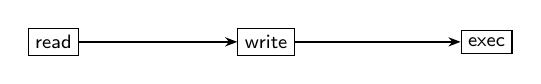
\begin{tikzpicture}[baseline=-0.55ex]
  \node[draw, font=\scriptsize\sffamily, inner sep=2.5pt] (r) at (0,0) {read};
  \node[draw, font=\scriptsize\sffamily, inner sep=2.5pt] (w) at (2.7,0) {write};
  \node[draw, font=\scriptsize\sffamily, inner sep=2.5pt] (e) at (5.5,0) {exec};
  \draw[arr] (r) -- (w);
  \draw[arr] (w) -- (e);
\end{tikzpicture}
\captionof{figure}{Permission order. Each permission includes the one to its left. A harness grant may move left along this order, or stay, and may not move right of the parent grant.}
\label{fig:perm}
\end{center}

HarnessSpec is the typed protocol for one harness. Version 0.1 is the version implemented here. The proposal states three objectives. O1 is the protocol. O2 is the compiler, the runtime, and revision of a spec from its trace. O3 is a comparison of four designers on about 60 SWE-bench Verified issue-resolution tasks and about 60 SWE-QA repository questions, using open-weight models in the 7--14B and 24--30B bands, three seeds, and energy reported beside accuracy. This report covers O1 and the part of O2 that runs without a model. Section~\ref{sec:hyp} restates the four pre-registered hypotheses and separates them from the fixture measurements.

\begin{figure}[H]
\centering
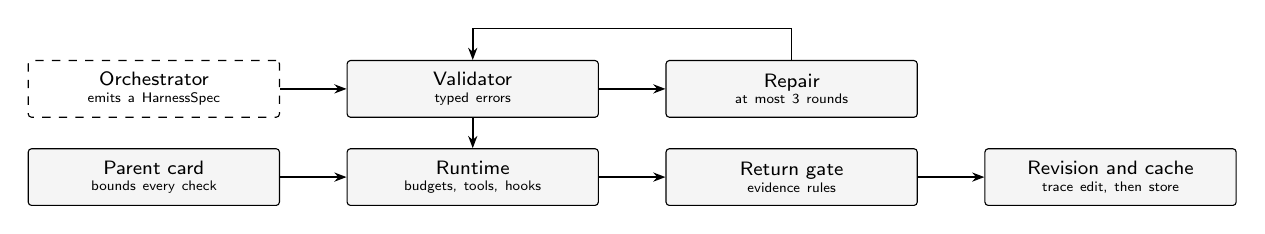
\begin{tikzpicture}[x=4.05cm, y=1.12cm]
  \node[later, text width=3.05cm] (orch) at (0,1) {Orchestrator\\[-2pt]{\tiny emits a HarnessSpec}};
  \node[flow, text width=3.05cm] (val) at (1,1) {Validator\\[-2pt]{\tiny typed errors}};
  \node[flow, text width=3.05cm] (rep) at (2,1) {Repair\\[-2pt]{\tiny at most 3 rounds}};
  \node[flow, text width=3.05cm] (card) at (0,0) {Parent card\\[-2pt]{\tiny bounds every check}};
  \node[flow, text width=3.05cm] (run) at (1,0) {Runtime\\[-2pt]{\tiny budgets, tools, hooks}};
  \node[flow, text width=3.05cm] (gate) at (2,0) {Return gate\\[-2pt]{\tiny evidence rules}};
  \node[flow, text width=3.05cm] (rev) at (3,0) {Revision and cache\\[-2pt]{\tiny trace edit, then store}};
  \draw[arr] (orch) -- (val);
  \draw[arr] (val) -- (rep);
  \draw[arr] (rep.north) -- ($(rep.north)+(0,4mm)$) -| (val.north);
  \draw[arr] (val) -- (run);
  \draw[arr] (card) -- (run);
  \draw[arr] (run) -- (gate);
  \draw[arr] (gate) -- (rev);
\end{tikzpicture}
\caption{Pipeline for this snapshot. Solid boxes run in the repository. The dashed box is the orchestrator, which is not called. The upper arrow returns a repaired spec to the validator. A valid spec enters the runtime, which checks it against the parent card.}
\label{fig:pipeline}
\end{figure}

\section{Scope of the measurements}
\label{sec:scope}

A fixture pilot is a run on a workspace whose correct behaviour is known, with actions supplied by the test rather than by a model. Every number in Sections~\ref{sec:compiler} and~\ref{sec:runtime} comes from \texttt{pilot/results.json}, produced by \texttt{pilot/run\_pilot.py} on Python 3.12.10. The unit tests re-run that script and fail if the file differs.

\begin{table}[H]
\centering
\small
\begin{tabularx}{\textwidth}{@{}YlY@{}}
\toprule
Component & Objective & State \\
\midrule
Protocol, eight fields, version 0.1 & O1 & Implemented. The schema and the validator name the same top-level fields. \\
Validator and repair & O2 & Implemented. Measured on 15 specs. \\
Budgets, tool guards, hooks, return gate & O2 & Implemented on one scripted workspace. \\
Trace revision and the spec cache & O2 & Implemented. The break-even task count is not computed. \\
Designers A and the four-field form of C & Preparation for O3 & A runs on the fixture. C is a partial object. No model is called. \\
Designer B and a live orchestrator & O3 & Not run. \\
SWE-bench Verified, SWE-QA, seeds, energy & O3 & Not run. \\
\bottomrule
\end{tabularx}
\end{table}

\section{Protocol}

A HarnessSpec is one JSON object. \texttt{spec\_version} and \texttt{task\_id} identify the object. The eight fields are the harness.

\begin{table}[H]
\centering
\small
\begin{tabularx}{\textwidth}{@{}lY@{}}
\toprule
Field & Requirement \\
\midrule
\texttt{goal} & A non-empty statement, and at least one acceptance test whose command is on the runtime allowlist. \\
\texttt{context} & Include-paths inside the parent slice. Absolute paths and \texttt{..} are rejected. \\
\texttt{tools} & The name exists on the parent card. The permission respects Figure~\ref{fig:perm}. Each path lies inside that tool's prefix. \\
\texttt{budgets} & Steps, tokens, and seconds are at least 1 and at most the parent card. Tokens cover one token per step. \\
\texttt{stop} & The stop conditions are from a fixed set. On exhaustion the harness stops or escalates. \\
\texttt{verification} & Hooks of kind \texttt{test}, \texttt{lint}, or \texttt{ast}. The command matches the kind. \\
\texttt{return\_contract} & If citations are required, the contract demands at least one. \\
\texttt{model} & The tier is \texttt{7-14B} or \texttt{24-30B}, and the parent card lists that tier. \\
\bottomrule
\end{tabularx}
\end{table}

The verification allowlist contains three commands, \texttt{unittest}, \texttt{ast.parse}, and \texttt{lint.bare-except}. Acceptance tests use the same list. The runtime implements these three and no others, so a check can accept or refuse a command by name. A shell string is not a command in the protocol. The benchmark phase can add further named commands for SWE-bench Verified. Each added command will be an entry the runtime implements, as these three are.

\texttt{examples/valid\_spec.json} validates against \texttt{examples/parent.json}. It is designer~D for the adder in Section~\ref{sec:runtime}: the goal is to make \texttt{add} return the sum of its arguments; the tools are \texttt{read\_file} and \texttt{write\_file} on \texttt{src}; the budgets are 6 steps, 2000 tokens, and 30 seconds; the hooks are \texttt{unittest} and \texttt{ast.parse}; the return contract requires a citation and test output; the tier is \texttt{7-14B}. A unit test builds A and D and requires both to validate.

The four designers are named here so the later sections can use the letters. Designer~A is a fixed harness: every tool on the parent card, the parent's budgets, an empty hook list, and no citation requirement. Designer~D is the harness in the example file, with a tighter step budget where a test needs one. Designer~C is the four-field tuple of instruction, context paths, tool names, and model name, without budgets, stop rules, verification, or a return contract. Designer~B is a free-text brief. The brief is stored as text. The compiler in this snapshot accepts HarnessSpec objects, so B is retained for the later study and is not passed through the validator.

\section{Compiler}
\label{sec:compiler}

The validator is a function of the spec and the parent card. It returns a sorted list of typed errors. It does not read a clock and does not call a model. \texttt{schema/harnessspec.schema.json} is the interchange description of the same object. The Python validator is the check the runtime executes. A unit test requires the two descriptions to require the same top-level fields.

Repair consumes that error list and writes a new spec. It runs for at most three rounds and stops earlier when a round leaves the spec unchanged. Repair may delete an unknown field, drop an unknown tool, lower a permission to the parent grant, clamp a budget to the parent card, and supply a missing budget, stop rule, hook list, or return contract from a fixed default. The default return contract requires citations and test output, and the default stop rule escalates when the budget is exhausted. Repair does not write goal text, an acceptance test, or a context path. Those three items are the statement of the task. A default would put words in the spec that no writer supplied. The parent card used for the corpus grants \texttt{read\_file} (read on \texttt{src}, \texttt{tests}, and \texttt{README.md}), \texttt{write\_file} (write on \texttt{src}), \texttt{list\_dir} (read on the workspace), and \texttt{run\_tests} (exec on \texttt{tests}), with 30 steps, 8000 tokens, 120 seconds, and both model tiers.

\begin{table}[H]
\centering
\footnotesize
\begin{tabularx}{\textwidth}{@{}YccY@{}}
\toprule
Spec & Initial & After repair & Result \\
\midrule
Four well-formed harnesses & valid & unchanged & Left as written. \\
Unknown tool; exec on a write-only tool; budget above the parent; tokens below the step count; tier \texttt{70B}; an extra field; a write path outside \texttt{src} & invalid & valid in 1 round & The tool is dropped, the permission is lowered, the budget is clamped, or the field is deleted. \\
Empty acceptance list & invalid & still invalid & \texttt{goal.acceptance\_tests} remains. \\
Blank goal statement & invalid & still invalid & \texttt{goal.empty} remains. \\
Include path \texttt{../secrets} & invalid & stops at round 2 & The path is removed. The slice is then empty, and no path is added. \\
Designer~C tuple & invalid & stops at round 2 & Budgets, stop, verification, return contract, and tier are filled from the defaults. The remaining error is the missing acceptance test. \\
\bottomrule
\end{tabularx}
\end{table}

Fifteen specs were validated. Four were valid on the first pass. Seven became valid in one repair round. Four remained invalid, and none of the fifteen used the third round. The unknown-tool spec was validated 100 times and produced one verdict, \texttt{tool.unknown}.

The tuple row is a property of this compiler. The first pass reports missing budgets, stop rules, verification, return contract, model tier, and acceptance tests. Repair fills the five fields that have defaults and stops with \texttt{schema.missing} at \texttt{goal.acceptance\_tests}. The object repair emits is not designer~C. In the comparison study, designer~C is the tuple as emitted, before repair. Repairing C until it matched D would remove the contrast the study is designed to measure.

\section{Runtime}
\label{sec:runtime}

The runtime refuses a spec that the validator rejects. Figure~\ref{fig:checks} is the order of checks on one action.

\begin{figure}[H]
\centering
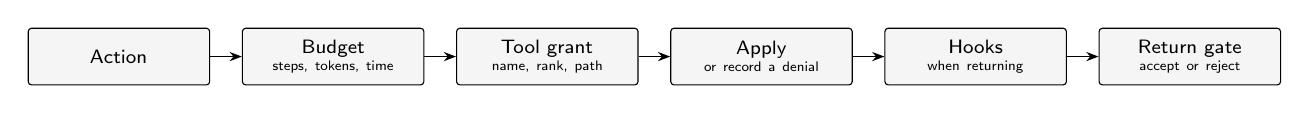
\begin{tikzpicture}[x=2.72cm]
  \node[chk, text width=2.15cm] (act) at (0,0) {Action};
  \node[chk, text width=2.15cm] (bud) at (1,0) {Budget\\[-2pt]{\tiny steps, tokens, time}};
  \node[chk, text width=2.15cm] (tool) at (2,0) {Tool grant\\[-2pt]{\tiny name, rank, path}};
  \node[chk, text width=2.15cm] (app) at (3,0) {Apply\\[-2pt]{\tiny or record a denial}};
  \node[chk, text width=2.15cm] (hook) at (4,0) {Hooks\\[-2pt]{\tiny when returning}};
  \node[chk, text width=2.15cm] (gate) at (5,0) {Return gate\\[-2pt]{\tiny accept or reject}};
  \draw[arr] (act) -- (bud);
  \draw[arr] (bud) -- (tool);
  \draw[arr] (tool) -- (app);
  \draw[arr] (app) -- (hook);
  \draw[arr] (hook) -- (gate);
\end{tikzpicture}
\caption{Checks on one action, in order. A budget miss stops the run. A tool miss is logged and the action is not applied. Hooks and the return gate run when the action is a return.}
\label{fig:checks}
\end{figure}

Time is read from a clock passed into the runtime. In the fixture the clock advances by the duration written on the action. The budget decision is then determined by the spec and the script. A wall-clock implementation is in the runtime for a later live run. The figures below use the fixture clock.

A tool call must name a tool on the harness allowlist, use a permission at or below the harness permission, and name a path inside the granted prefix. Otherwise the call is a denial and has no effect on the workspace. A return runs the hooks and then the return gate. The gate accepts the result when every evidence rule in the contract holds. A silent handoff is an accepted return whose summary is non-empty and which carries no usable \texttt{file:line} citation. A rejected return is recorded as a rejection. It is not counted as a silent handoff.

The workspace \texttt{fixtures/off\_by\_one} contains \texttt{src/app.py}, which returns \texttt{a + b + 1}, and a test that expects \texttt{a + b}. The same scripted actions were given to designer~A and designer~D. No model selected the actions.

\begin{table}[H]
\centering
\footnotesize
\begin{tabularx}{\textwidth}{@{}Y YY@{}}
\toprule
Scripted task & Designer A & Designer D \\
\midrule
Patch the file, then return ``the bug is fixed'' with no citation & Accepted. Silent handoff. No hooks ran. & Both hooks passed. The return was rejected. \\
Three writes; D is capped at 2 steps & All three writes applied. & The third write was intercepted. One budget violation. Two steps used. Stop action: escalate. \\
Call \texttt{run\_tests} as \texttt{exec} & Applied. The parent card allows it, and A grants it. & One tool denial. D does not grant an exec tool. \\
Return a cited claim while the test still fails & Accepted. Hooks were not run. & Rejected. \texttt{unittest} failed. Stop code: \texttt{hook\_failed}. \\
Patch the file, then return \texttt{src/app.py:2} and test output & A does not consult the test. & Both hooks passed. The return was accepted. \\
\bottomrule
\end{tabularx}
\end{table}

On the first row the patch was applied under both designers, and the test was able to pass. A accepted a summary with no citation. D ran both hooks and rejected the summary. On the fourth row the file was still wrong: A accepted a cited claim without running the test, and D rejected the return after \texttt{unittest} failed. On the fifth row D accepted the return after the test passed and the citation and test output were present. These nine runs, on one workspace and one seed, define the silent-handoff bit, the budget-violation count, the tool-denial count, and the hook failure. Designers B and C were not executed.

Revision reads a trace and may raise \texttt{max\_steps}. The new cap is the minimum of the parent cap and the larger of two candidates: the old cap plus two steps, and one and a half times the old cap. The token budget is raised to match when the parent card allows it. Revision does not add a tool the spec withheld, and it does not clear a citation requirement. The trace can draw on parent budget the spec has not yet used. It cannot change the evidence the contract demands. On a harness capped at 2 steps, the third action was a budget violation. Revision raised the cap from 2 to 4. \texttt{require\_citations} stayed true and \texttt{min\_citations} stayed 1. The revised spec validates.

The spec cache stores a validated spec under a key of task type and model tier. A second lookup with the same key returns the stored spec and does not enter repair. The fixture recorded one miss and one hit for task type \texttt{bugfix} at tier \texttt{7-14B}. The break-even count in H4 is the number of tasks at which a cached spec pays for the design call. No design call was made, so that count is not defined for this snapshot. The repairer used above is deterministic.

\section{Registered hypotheses}
\label{sec:hyp}

The proposal fixes four hypotheses and states that a negative result is reported as a negative result. The hypotheses are unchanged. The table pairs each claim with the instrument this snapshot provides and with the quantity still required.

\begin{table}[H]
\centering
\footnotesize
\begin{tabularx}{\textwidth}{@{}>{\hsize=1.25\hsize}Y>{\hsize=0.95\hsize}Y>{\hsize=0.8\hsize}Y@{}}
\toprule
 & Instrument now available & Still required \\
\midrule
H1. D stays within 5 points of A on accuracy and uses fewer tokens, with the design call included. & A and D both run on a scripted task. & Accuracy, model tokens, and a design call. \\
H2. D has fewer silent handoffs than B and C. & The silent-handoff bit. On the fixture, A accepts a summary with no citation and D rejects it. & Runs of B and C, and returns written by a model. \\
H3. Validation and revision raise first-pass validity, most for a 7--14B orchestrator. & Typed errors, a three-round cap, and a count on 15 hand-written specs. & An orchestrator. \\
H4. Report how many tasks a cached spec must cover before the design call is paid for. & A cache, with one miss and one hit. & A design-call cost above zero. \\
\bottomrule
\end{tabularx}
\end{table}

H1 fails if D trails A by more than 5 points. H2 fails if D's silent-handoff rate is not lower than the rates for B and C. H3 fails if first-pass validity does not rise, including when an orchestrator rarely emits an acceptance test. H4 fails if the design call is not recovered inside the task set. Repair is not applied afterwards to turn any of these outcomes into a pass.

\section{Repository}

The implementation is at \url{https://github.com/GauravSarkarr/HarnessSpec}.

The commits of 5 November 2026, in build order, are \texttt{5ec1ef5} (schema, path rules, and the parent card), \texttt{e3ea1db} (validator), \texttt{47c8a7a} (repair), \texttt{aca97ab} (runtime, hooks, and the return gate), \texttt{02c1967} (designers A and C, and revision), \texttt{a60e33e} (fixture pilot and the test that re-runs it), and \texttt{aa8204d} (README and the AI-use log).

From a clean checkout, with no installed packages:

{\footnotesize\ttfamily
\begin{flushleft}
PYTHONPATH=src python3 -m unittest discover -s tests -v\\
PYTHONPATH=src python3 pilot/run\_pilot.py\\
PYTHONPATH=src python3 -m harnessspec \\
examples/valid\_spec.json examples/parent.json
\end{flushleft}
}

\noindent The test suite re-runs the pilot and fails if the committed results differ.

\noindent The source of this report is \texttt{mid\_submission.tex}.

The proposal requires a log of AI-tool use. On 5 November 2026, Cursor, using Grok 4.7, drafted the milestone implementation and this report. The check is the test command above. No orchestrator model and no subagent model were called. The log is \texttt{AI\_USE.md}.

\section{Remaining work}

The second half is the study registered in the proposal.
\begin{enumerate}
\item One 7--14B model emits a HarnessSpec. Typed errors are returned to it for at most three rounds. The recorded quantities are the first-pass validity rate and the number of rounds. That run is a pilot for H3.
\item Designers B and C are run as specified. B remains a free-text brief. C remains the four-field tuple, scored before repair, so a missing acceptance test is a property of the emitted tuple. D is the full spec plus the validator.
\item Ten SWE-bench Verified instances pass through the edit-and-test loop before the registered sizes of about 60 and about 60. Those ten determine which named commands the allowlist must gain. SWE-QA follows once that slice runs.
\item Tokens are taken from the server, with the design call included. Three seeds and paired bootstrap intervals are reported. CPU and GPU energy are reported beside accuracy. The H4 break-even is computed once a design call has a token cost.
\item The hook allowlist grows by the named commands those benchmarks require.
\end{enumerate}

Two limits follow from the mechanisms above. A missing acceptance test is left in place, so a 7--14B orchestrator that rarely emits one yields a low first-pass validity for D, which is the H3 measurement. The fixture hook is \texttt{unittest} in one workspace, while SWE-bench Verified uses other commands, so the runtime can be correct on this fixture and still need new allowlist entries. The next measurement is therefore ten instances. This report contains no success rate per kilowatt-hour and no token count per correct answer.

\section{Status}

O1 is implemented: HarnessSpec 0.1 is an eight-field protocol with a deterministic validator. The part of O2 that does not require a model is implemented on the fixture: budgets, tool grants, hooks, and the return gate determine which scripted actions are applied and which returns are accepted, and repair leaves the task statement unchanged. O3 has not been run. H1--H4 are not results of this report.

\end{document}
